<<<<<<< HEAD
\documentclass{article}
\usepackage[english]{babel}
\usepackage[letterpaper,top=2cm,bottom=2cm,left=3cm,right=3cm,marginparwidth=1.75cm]{geometry}
\usepackage{amsmath}
\usepackage{graphicx}
\usepackage{algorithm}
\usepackage{algorithmicx}
\usepackage{algpseudocode}
\usepackage{forest}
\usepackage{setspace}
\usepackage{tikz}
\usepackage[colorlinks=true, allcolors=blue]{hyperref}

\title{\textbf{CS456: Algorithm Design and Analysis}}
\author{Elikem Asudo Tsatsu Gale-Zoyiku}
\date{\today}

\begin{document}
\doublespacing
\maketitle
\begin{center}
    \begin{large}
        \textbf{Assignment 4\\}
    \end{large}
\end{center}
\newpage

\section*{Problem 1 (Prim's Algorithm)}
\begin{table}[ht]
    \centering
    \begin{tabular}{|c|c|}
        \hline
        \textbf{Tree Vertices} & \textbf{Remaining Vertices}                                                                          \\
        \hline
        a(-,-)                 & b(a,3) c(a,5) d(a,4) $e(-,\infty)$ $f(-,\infty)$ $g(-,\infty)$ $h(-,\infty)$                         \\
                               & $i(-,\infty)$ $j(-,\infty)$ $k(-,\infty)$ $l(-,\infty)$                                              \\
        \hline
        b(a,3)                 & e(b, 3) f(b, 6) $c(a,5)$ $d(a,4)$ $g(-,\infty)$ $h(-,\infty)$                                        \\
                               & $i(-,\infty)$ $j(-,\infty)$ $k(-,\infty)$ $l(-,\infty)$                                              \\
        \hline
        e(b,3)                 & f(e, 2) d(e, 1) i(e, 4) c(a,5) $g(-,\infty)$ $h(-,\infty)$ $j(-,\infty)$ $k(-,\infty)$ $l(-,\infty)$ \\
        \hline
        d(e,1)                 & f(e,2) i(e,4) c(d,2) $g(-,\infty)$ h(d, 5) $j(-,\infty)$ $k(-,\infty)$ $l(-,\infty)$                 \\
        \hline
        c(d,2)                 & f(e,2) i(e,4) g(c, 4) h(d,5) $j(-,\infty)$ $k(-,\infty)$ $l(-,\infty)$                               \\
        \hline
        f(e,2)                 & i(e,4) g(c,4) h(d,5) j(f, 5) $k(-,\infty)$ $l(-,\infty)$                                             \\
        \hline
        i(e,4)                 & g(c,4) h(d,5) j(i,3) l(i, 5) $k(-,\infty)$                                                           \\
        \hline
        j(i,3)                 & g(c,4) h(d,5) l(i,5) $k(-,\infty)$                                                                   \\
        \hline
        g(c,4)                 & h(g,3) l(i,5) k(g, 6)                                                                                \\
        \hline
        h(g,3)                 & l(i,5) k(g,6)                                                                                        \\
        \hline
        l(i,5)                 & k(g,6)                                                                                               \\
        \hline
        k(g,6)                 &                                                                                                      \\
        \hline
    \end{tabular}
    \caption{Prim's Algorithm to produce minimum spanning tree}
    \label{tab:my_table}
\end{table}

\begin{figure}[h]
    \centering
    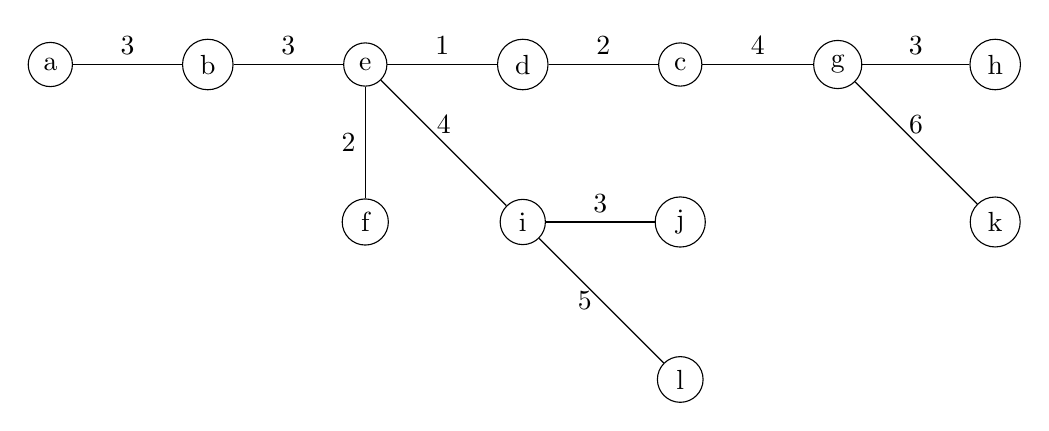
\begin{tikzpicture}
        \node[draw,circle] (a) at (0,0) {a};
        \node[draw,circle] (b) at (2,0) {b};
        \node[draw,circle] (e) at (4,0) {e};
        \node[draw,circle] (d) at (6,0) {d};
        \node[draw,circle] (c) at (8,0) {c};
        \node[draw,circle] (f) at (4,-2) {f};
        \node[draw,circle] (i) at (6,-2) {i};
        \node[draw,circle] (j) at (8,-2) {j};
        \node[draw,circle] (g) at (10,0) {g};
        \node[draw,circle] (h) at (12,0) {h};
        \node[draw,circle] (l) at (8,-4) {l};
        \node[draw,circle] (k) at (12,-2) {k};

        \draw (a) -- node[above] {3} (b);
        \draw (b) -- node[above] {3} (e);
        \draw (e) -- node[above] {1} (d);
        \draw (d) -- node[above] {2} (c);
        \draw (e) -- node[left] {2} (f);
        \draw (e) -- node[above] {4} (i);
        \draw (i) -- node[above] {3} (j);
        \draw (c) -- node[above] {4} (g);
        \draw (g) -- node[above] {3} (h);
        \draw (i) -- node[left] {5} (l);
        \draw (g) -- node[above] {6} (k);
    \end{tikzpicture}
    \caption{Minimum Spanning Tree generated using Prim's Algorithm}
\end{figure}

\newpage

\section*{Problem 2 (Kruskal's Algorithm)}
\begin{table}[ht]
    \centering
    \begin{tabular}{|c|c|}
        \hline
        \textbf{Tree Edges} & \textbf{Sorted List of Edges}                               \\
        \hline
                            & de(1) cd(2) ef(2) ab(3) be(3) gh(3) ij(3) ad(4) cg(4) ei(4) \\
                            & ac(5) dh(5) fj(5) il(5) bf(6) gk(6) hi(6) hk(7) kl(8) jl(9) \\
        \hline
        de(1)               & cd(2) ef(2) ab(3) be(3) gh(3) ij(3) ad(4) cg(4) ei(4)       \\
                            & ac(5) dh(5) fj(5) il(5) bf(6) gk(6) hi(6) hk(7) kl(8) jl(9) \\
        \hline
        cd(2)               & ef(2) ab(3) be(3) gh(3) ij(3) ad(4) cg(4) ei(4)             \\
                            & ac(5) dh(5) fj(5) il(5) bf(6) gk(6) hi(6) hk(7) kl(8) jl(9) \\
        \hline
        ef(2)               & ab(3) be(3) gh(3) ij(3) ad(4) cg(4) ei(4)                   \\
                            & ac(5) dh(5) fj(5) il(5) bf(6) gk(6) hi(6) hk(7) kl(8) jl(9) \\
        \hline
        ab(3)               & be(3) gh(3) ij(3) ad(4) cg(4) ei(4)                         \\
                            & ac(5) dh(5) fj(5) il(5) bf(6) gk(6) hi(6) hk(7) kl(8) jl(9) \\
        \hline
        be(3)               & gh(3) ij(3) ad(4) cg(4) ei(4)                               \\
                            & ac(5) dh(5) fj(5) il(5) bf(6) gk(6) hi(6) hk(7) kl(8) jl(9) \\
        \hline
        gh(3)               & ij(3) ad(4) cg(4) ei(4)                                     \\
                            & ac(5) dh(5) fj(5) il(5) bf(6) gk(6) hi(6) hk(7) kl(8) jl(9) \\
        \hline
        ij(3)               & ad(4) cg(4) ei(4)                                           \\
                            & ac(5) dh(5) fj(5) il(5) bf(6) gk(6) hi(6) hk(7) kl(8) jl(9) \\
        \hline
        cg(4)               & ad(4) ei(4)                                                 \\
                            & ac(5) dh(5) fj(5) il(5) bf(6) gk(6) hi(6) hk(7) kl(8) jl(9) \\
        \hline
        ei(4)               & ad(4)                                                       \\
                            & ac(5) dh(5) fj(5) il(5) bf(6) gk(6) hi(6) hk(7) kl(8) jl(9) \\
        \hline
        il(5)               & dh(5) fj(5)                                                 \\
                            & ac(5) bf(6) gk(6) hi(6) hk(7) kl(8) jl(9)                   \\
        \hline
        gk(6)               & hi(6) hk(7)                                                 \\
                            & ac(5) bf(6) kl(8) jl(9)                                     \\
        \hline
    \end{tabular}
    \caption{Kruskal's Algorithm to produce minimum spanning tree}
    \label{tab:table2}
\end{table}

\begin{figure}[h]
    \centering
    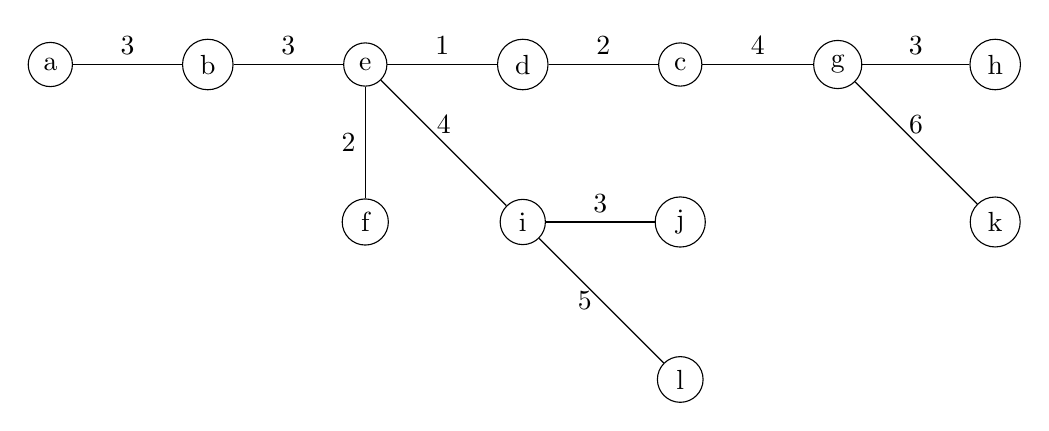
\begin{tikzpicture}
        \node[draw,circle] (a) at (0,0) {a};
        \node[draw,circle] (b) at (2,0) {b};
        \node[draw,circle] (e) at (4,0) {e};
        \node[draw,circle] (d) at (6,0) {d};
        \node[draw,circle] (c) at (8,0) {c};
        \node[draw,circle] (f) at (4,-2) {f};
        \node[draw,circle] (i) at (6,-2) {i};
        \node[draw,circle] (j) at (8,-2) {j};
        \node[draw,circle] (g) at (10,0) {g};
        \node[draw,circle] (h) at (12,0) {h};
        \node[draw,circle] (l) at (8,-4) {l};
        \node[draw,circle] (k) at (12,-2) {k};

        \draw (a) -- node[above] {3} (b);
        \draw (b) -- node[above] {3} (e);
        \draw (e) -- node[above] {1} (d);
        \draw (d) -- node[above] {2} (c);
        \draw (e) -- node[left] {2} (f);
        \draw (e) -- node[above] {4} (i);
        \draw (i) -- node[above] {3} (j);
        \draw (c) -- node[above] {4} (g);
        \draw (g) -- node[above] {3} (h);
        \draw (i) -- node[left] {5} (l);
        \draw (g) -- node[above] {6} (k);
    \end{tikzpicture}
    \caption{Minimum Spanning Tree generated using Kruskal's Algorithm}
\end{figure}

\newpage

\section*{Problem 3 (Djikstra's Algorithm)}
\begin{table}[ht]
    \centering
    \begin{tabular}{|c|c|}
        \hline
        \textbf{Tree Vertices} & \textbf{Remaining Vertices}                                                                                                          \\
        \hline
        a(-,0)                 & b(a,3) c(a,5) d(a,4) e(-,$\infty$) f(-,$\infty$) g(-,$\infty$) h(-,$\infty$) i(-,$\infty$) j(-,$\infty$) k(-,$\infty$) l(-,$\infty$) \\
        \hline
        b(a,3)                 & e(b,3+3) f(b,3+6) c(a,5) d(a,4) g(-,$\infty$) h(-,$\infty$) i(-,$\infty$) j(-,$\infty$) k(-,$\infty$) l(-,$\infty$)                  \\
        \hline
        d(a,4)                 & e(d,4+1) f(b,9) c(a,5) g(-,$\infty$) h(d,4+5) i(-,$\infty$) j(-,$\infty$) k(-,$\infty$) l(-,$\infty$)                                \\
        \hline
        c(a,5)                 & e(d,5) f(b,9) g(c,5+4) h(d,9) i(-,$\infty$) j(-,$\infty$) k(-,$\infty$) l(-,$\infty$)                                                \\
        \hline
        e(d,5)                 & f(e,5+2 == 7) g(c,9) h(d,9) i(-,5+4 == 9) j(-,$\infty$) k(-,$\infty$) l(-,$\infty$)                                                  \\
        \hline
        f(e,7)                 & g(c,9) h(d,9) i(e,9) j(f,7+5) k(-,$\infty$) l(-,$\infty$)                                                                            \\
        \hline
        g(c,9)                 & h(d,9) i(e,9) j(f,12) k(g,9+6) l(-,$\infty$)                                                                                         \\
        \hline
        h(d,9)                 & i(e,9) j(f,12) k(g,15) l(-,$\infty$)                                                                                                 \\
        \hline
        i(e,9)                 & j(f,12) k(g,15) l(i,9+5)                                                                                                             \\
        \hline
        j(f,12)                & k(g,15) l(i,14)                                                                                                                      \\
        \hline
        l(i,14)                & k(g,15)                                                                                                                              \\
        \hline
        k(g,15)                &                                                                                                                                      \\
        \hline
    \end{tabular}
    \caption{Djikstra's Algorithm to find shortst path to each vertex from source a}
    \label{tab:table3}
\end{table}
\textbf{Shortest Paths from a to each vertex:}
\begin{itemize}
    \item from a to b : a $\rightarrow$ b of length 3
    \item from a to d : a $\rightarrow$ d of length 4
    \item from a to c : a $\rightarrow$ c of length 5
    \item from a to e : a $\rightarrow$ d $\rightarrow$ e of length 5
    \item from a to f : a $\rightarrow$ d $\rightarrow$ e $\rightarrow$ f of length 7
    \item from a to g : a $\rightarrow$ c $\rightarrow$ g of length 9
    \item from a to h : a $\rightarrow$ d $\rightarrow$ h of length 9
    \item from a to i : a $\rightarrow$ d $\rightarrow$ e $\rightarrow$ i of length 9
    \item from a to j : a $\rightarrow$ d $\rightarrow$ e $\rightarrow$ f $\rightarrow$ j of length 12
    \item from a to l : a $\rightarrow$ d $\rightarrow$ e $\rightarrow$ i $\rightarrow$ l of length 14
    \item from a to k : a $\rightarrow$ c $\rightarrow$ g $\rightarrow$ k of length 15
\end{itemize}
\newpage
\section*{Problem 4}
\subsection*{a}
No adjustments are needed to Djikstra's Algorithm to find the shortest path in a directed graph.
All nodes in the directed graph would have edges, and costs, to and from them. The algorithm would
work as expected by exploring those edges and costs. In implementing it, just like with undirected
graphs, the graph would be represented with each node having a list of connections to other nodes
and the costs of those connections. However, unlike in an undirected graph where each edge is essentially
a two-way connection between nodes, in a directed graph, connections are not duplicated. This means that
an edge from node A to node B does not imply an edge from node B to node A.

\subsection*{b}
The algorithm would have to be adjusted to start at the source vertex as usual.
Instead of terminating when all vertices have been visited, terminate the algorithm
when the target vertex is reached, and there no more paths ending at the target vertex.
Determine the shortest path to the target vertex. Every
other part of the algorithm would work the same (calculating the displacement from the source vertex).
However, early pruning could be factored in to avoid exploring nodes that are not on the path to the target vertex (e.g. dead ends).
\\
\subsection*{c}
The algorithm would have to be adjusted to start at the source vertex as usual,
and terminate when there are no more edges to the target vertex. The algorithm would also have to be
adjusted to iterate over all the vertices in the graph, setting each one as the source,
and for each vertex,
find the shortest path to the target vertex. For each complete run through,
the shortest path is determined.

\subsection*{d}
To adapt Dijkstra's algorithm for solving the single-source shortest-paths problem in a graph with nonnegative numbers assigned to its vertices, where the length of a path is defined as the sum of the vertex numbers on the path, the following adjustments are needed:
\begin{enumerate}
    \item Instead of traditional edge weights, use the sum of vertex numbers along the path as the weight of each edge.
    \item Initialize the algorithm by setting the source vertex and assigning a distance of zero to it. Set the distances of all other vertices to infinity.
    \item Select the vertex with the smallest cumulative vertex number sum as the next vertex to explore.
    \item Update the distance to each vertex based on the cumulative vertex number sum along the path to that vertex. If the cumulative sum through a vertex is smaller than the current known distance to that vertex, update the distance accordingly.
    \item Termination: Terminate the algorithm when all vertices have been visited. The shortest path to each vertex will be the path with the smallest cumulative vertex number sum.
\end{enumerate}
\newpage
\section*{Problem 5}
\subsection*{Bottom-Up Approach to the Knapsack Problem}
\begin{table}[ht]
    \centering
    Capacity $j$

    \begin{tabular}{c|c|c|c|c|c|c|c|c|c|}
        \hline
        \textbf{Item $i$}           & \textbf{0} & \textbf{1} & \textbf{2} & \textbf{3} & \textbf{4} & \textbf{5} & \textbf{6} & \textbf{7} & \textbf{8} \\
        \hline
        0                           & 0          & 0          & 0          & 0          & 0          & 0          & 0          & 0          & 0          \\
        \hline
        Item 1 | $w_1 = 1, v_1 = 2$ & 0          & 2          & 2          & 2          & 2          & 2          & 2          & 2          & 2          \\
        \hline
        Item 2 | $w_2 = 2, v_2 = 4$ & 0          & 2          & 4          & 6          & 6          & 6          & 6          & 6          & 6          \\
        \hline
        Item 3 | $w_3 = 3, v_3 = 5$ & 0          & 2          & 4          & 6          & 7          & 9          & 11         & 11         & 11         \\
        \hline
        Item 4 | $w_4 = 4, v_4 = 5$ & 0          & 2          & 4          & 6          & 7          & 9          & 11         & 11         & 12         \\
        \hline
        Item 5 | $w_5 = 2, v_5 = 2$ & 0          & 2          & 4          & 6          & 7          & 9          & 11         & 11         & 13         \\
        \hline
        Item 6 | $w_6 = 1, v_6 = 3$ & 0          & 3          & 5          & 7          & 9          & 10         & 12         & 14         & 14         \\
        \hline
    \end{tabular}
    \caption{Table for the Bottom-Up Approach to the Knapsack Problem}
    \label{tab:table4}
\end{table}

\subsection*{a}
The optimal solution to this instance of the knapsack problem is 14. The optimal subset can be found by:
\begin{itemize}
    \item 14 - Profit of item 6 $\rightarrow$ 14 - 3 = 11
    \item 11 - Profit of Item in row of first appearance of 11 $\rightarrow$ 11 - 5 = 6
    \item 6 - Profit of Item in row of first appearance of 6 $\rightarrow$ 6 - 4 = 2
    \item 2 - Profit of Item in row of first appearance of 2 $\rightarrow$ 2 - 2 = 0
\end{itemize}
The optimal subset is $\{Item 1, Item 2, Item 3, Item 6\}$ with cooresponding weights $\{1, 3, 2, 1\}$
and corresponding profits $\{2, 4, 5, 3\}$.

\subsection*{b}
To determine if there are multiple optimal subsets,
we can look at the table generated by the algorithm.
The value in the cell at the last row and last column of the table
is the optimal value of the knapsack problem. You would begin
backtracking from this cell to determine the optimal subset, i.e.
subtract the profit of the item in the row of the cell from the optimal value
and move to the cell in the row of the first appearance of the result.
Repeat this process until you reach the first row of the table.
If there are multiple optimal subsets, you would find that the
backtracking process would yield different subsets that have the same
optimal value, i.e. there would be multiple paths to the optimal value.
This could occur if there are multiple cells with the same profit value in the last column, i.e. mulitiple items
gave the same profit value. If there is only one optimal subset, the backtracking
process would yield only one subset.

\subsection*{c}
\begin{table}[ht]
    \centering
    Capacity $j$

    \begin{tabular}{c|c|c|c|c|c|c|c|c|c|}
        \hline
        \textbf{Item $i$}           & \textbf{0} & \textbf{1} & \textbf{2} & \textbf{3} & \textbf{4} & \textbf{5} & \textbf{6} & \textbf{7} & \textbf{8} \\
        \hline
        0                           & 0          & 0          & 0          & 0          & 0          & 0          & 0          & 0          & 0          \\
        \hline
        Item 1 | $w_1 = 1, v_1 = 2$ & 0          & 2          & 2          & 2          & 2          & 2          & 2          & 2          & 2          \\
        \hline
        Item 2 | $w_2 = 2, v_2 = 4$ & 0          & X          & 4          & 6          & 6          & 6          & 6          & 6          & 6          \\
        \hline
        Item 3 | $w_3 = 3, v_3 = 5$ & 0          & X          & X          & 6          & 7          & 9          & 11         & 11         & 11         \\
        \hline
        Item 4 | $w_4 = 4, v_4 = 5$ & 0          & X          & X          & X          & X          & X          & X          & 11         & 12         \\
        \hline
        Item 5 | $w_5 = 2, v_5 = 2$ & 0          & X          & X          & X          & X          & X          & X          & 11         & 13         \\
        \hline
        Item 6 | $w_6 = 1, v_6 = 3$ & 0          & X          & X          & X          & X          & X          & X          & X          & 14         \\
        \hline
    \end{tabular}
    \caption{Table for the Bottom-Up Approach to the Knapsack Problem with values never computed marked values never recomputed marked as X}
    \label{tab:table5}
\end{table}



\newpage
\section*{Problem 6}
\subsection*{a}
\begin{table}[ht]
    \centering
    \begin{tabular}{|c|c|}
        \hline
        \textbf{Tree Vertices} & \textbf{Remaining Vertices}                                     \\
        \hline
        A(-,0)                 & B(A,2) C(A,7) E(A,12) D(-,$\infty$) F(-,$\infty$) G(-,$\infty$) \\
        \hline
        B(A,2)                 & D(B,2+2) C(A,7) E(A,12) F(-,$\infty$) G(-,$\infty$)             \\
        \hline
        D(B,4)                 & C(A,7) E(A,12) F(D,4+2) G(-,$\infty$)                           \\
        \hline
        F(D,6)                 & C(A,7) E(A,12) G(F,8)                                           \\
        \hline
        C(A,7)                 & E(C,9) G(F,8)                                                   \\
        \hline
        G(F,8)                 & E(C,9)                                                          \\
        \hline
        E(C,9)                 &                                                                 \\
        \hline
    \end{tabular}
    \caption{Djikstra's Algorithm to find shortst path to each vertex from source a}
    \label{tab:table6}
\end{table}

\subsection*{c} Edge E-G

\newpage
\section*{Problem 7}
\begin{algorithm}
    \caption{Rod Cutting Algorithm}
    \begin{algorithmic}[1]
        \Procedure{rodCutting}{$n$, $prices$}
        \State Initialize memoization table $memo[0...n]$ with zeros
        \For{$i$ from 1 to $n$}
        \State $max\_price \gets -1$
        \For{$j$ from 1 to $i$}
        \State // Update $max\_price$ considering all possible cuts
        \State $max\_price \gets \max(max\_price, prices[j - 1] + memo[i - j])$
        \EndFor
        \State $memo[i] \gets max\_price$
        \EndFor
        \State \textbf{return} $memo[n]$  // Return the maximum sale price for a rod of length $n$
        \EndProcedure
    \end{algorithmic}
\end{algorithm}

\subsection*{Time Complexity}
The time complexity of this algorithm is $O(n^2)$.
The outer loop runs $n$ times (as many times as the length of the rod), and the inner loop runs $i$
times for each iteration of the outer loop, and $i$ ranges from 1 to $n$, so in the worst case, $i = n$. The operation being carried out is a
comparison and an addition operation, which are both $O(1)$ operations.
This gives a total of $T(n) = $ $\sum_{i=1}^{n}\sum_{i=1}^{i} O(1) = \sum_{i=1}^{n}\sum_{i=1}^{n} O(1) = \sum_{i=1}^{n}(n-1+1) = (n+1-1)(n) = O(n^2)$ iterations of the inner loop.

\subsection*{Space Complexity}
The space complexity of this algorithm is $O(n)$ as the memoization table $memo[0...n]$ has a size of $n$ where $n$ is the length of the rod.
As $n$ grows, the size of the memoization table grows linearly.
\newpage
\section*{Problem 8}
\subsection*{Graph 1}
\begin{itemize}
    \item Tour Edges: ('B', 'C'), ('A', 'B'), ('A', 'D'), ('B', 'D') (using multi-fragment heuristic)
    \item Minimum tour: ('C', 'B', 'A', 'D') with a total cost of 10
    \item Accuracy ratio = $AR = \sum(G[src][dest]) / Wmin, for all (src, dest) in E = \frac{3+2+5+4}{10} = 1.4$
\end{itemize}
\subsection*{Graph 2}
\begin{itemize}
    \item Tour Edges: ('A', 'B'), ('B', 'D'), ('A', 'C'), ('A', 'D') (using multi-fragment heuristic)
    \item Minimum tour: ('C', 'A', 'B', 'D') with a total cost of 50
    \item Accuracy ratio = $AR = \sum(G[src][dest]) / Wmin, for all (src, dest) in E = \frac{10+25+15+20}{50} = 1.4$
\end{itemize}
=======
\documentclass{article}
\usepackage[english]{babel}
\usepackage[letterpaper,top=2cm,bottom=2cm,left=3cm,right=3cm,marginparwidth=1.75cm]{geometry}
\usepackage{amsmath}
\usepackage{graphicx}
\usepackage{algorithm2e}
\usepackage{forest}
\usepackage{tikz}
\usepackage[colorlinks=true, allcolors=blue]{hyperref}

\title{\textbf{CS456: Algorithm Design and Analysis}}
\author{Elikem Asudo Tsatsu Gale-Zoyiku}
\date{\today}

\begin{document}
\maketitle
\begin{center}
    \begin{large}
        \textbf{Assignment 4\\}
    \end{large}
\end{center}
\newpage

\section*{Problem 1 (Prim's Algorithm)}
\begin{table}[ht]
    \centering
    \begin{tabular}{|c|c|}
        \hline
        \textbf{Tree Vertices} & \textbf{Remaining Vertices}                                                                                                          \\
        \hline
        a(-,-)                 & b(a,3) c(a,5) d(a,4) $e(-,\infty)$ $f(-,\infty)$ $g(-,\infty)$ $h(-,\infty)$ $i(-,\infty)$ $j(-,\infty)$ $k(-,\infty)$ $l(-,\infty)$ \\
        \hline
        b(a,3)                 & e(b, 3) f(b, 6) $c(a,5)$ $d(a,4)$ $g(-,\infty)$ $h(-,\infty)$ $i(-,\infty)$ $j(-,\infty)$ $k(-,\infty)$ $l(-,\infty)$                \\
        \hline
        e(b,3)                 & f(e, 2) d(e, 1) i(e, 4) c(a,5) $g(-,\infty)$ $h(-,\infty)$ $j(-,\infty)$ $k(-,\infty)$ $l(-,\infty)$                                 \\
        \hline
        d(e,1)                 & f(e,2) i(e,4) c(d,2) $g(-,\infty)$ h(d, 5) $j(-,\infty)$ $k(-,\infty)$ $l(-,\infty)$                                                 \\
        \hline
        c(d,2)                 & f(e,2) i(e,4) g(c, 4) h(d,5) $j(-,\infty)$ $k(-,\infty)$ $l(-,\infty)$                                                               \\
        \hline
        f(e,2)                 & i(e,4) g(c,4) h(d,5) j(f, 5) $k(-,\infty)$ $l(-,\infty)$                                                                             \\
        \hline
        i(e,4)                 & g(c,4) h(d,5) j(i,3) l(i, 5) $k(-,\infty)$                                                                                           \\
        \hline
        j(i,3)                 & g(c,4) h(d,5) l(i,5) $k(-,\infty)$                                                                                                   \\
        \hline
        g(c,4)                 & h(g,3) l(i,5) k(g, 6)                                                                                                                \\
        \hline
        h(g,3)                 & l(i,5) k(g,6)                                                                                                                        \\
        \hline
        l(i,5)                 & k(g,6)                                                                                                                               \\
        \hline
        k(g,6)                 &                                                                                                                                      \\
        \hline
    \end{tabular}
    \caption{Prim's Algorithm to produce minimum spanning tree}
    \label{tab:my_table}
\end{table}

\begin{figure}[h]
    \centering
    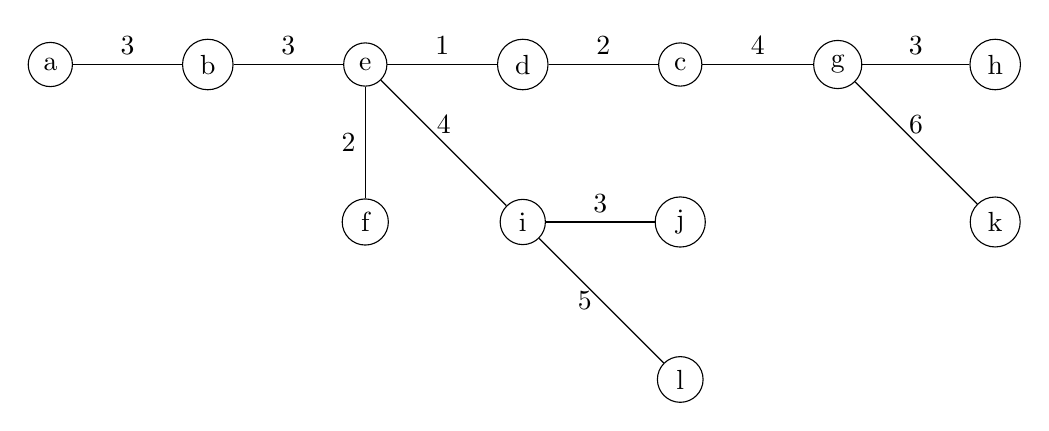
\begin{tikzpicture}
        \node[draw,circle] (a) at (0,0) {a};
        \node[draw,circle] (b) at (2,0) {b};
        \node[draw,circle] (e) at (4,0) {e};
        \node[draw,circle] (d) at (6,0) {d};
        \node[draw,circle] (c) at (8,0) {c};
        \node[draw,circle] (f) at (4,-2) {f};
        \node[draw,circle] (i) at (6,-2) {i};
        \node[draw,circle] (j) at (8,-2) {j};
        \node[draw,circle] (g) at (10,0) {g};
        \node[draw,circle] (h) at (12,0) {h};
        \node[draw,circle] (l) at (8,-4) {l};
        \node[draw,circle] (k) at (12,-2) {k};

        \draw (a) -- node[above] {3} (b);
        \draw (b) -- node[above] {3} (e);
        \draw (e) -- node[above] {1} (d);
        \draw (d) -- node[above] {2} (c);
        \draw (e) -- node[left] {2} (f);
        \draw (e) -- node[above] {4} (i);
        \draw (i) -- node[above] {3} (j);
        \draw (c) -- node[above] {4} (g);
        \draw (g) -- node[above] {3} (h);
        \draw (i) -- node[left] {5} (l);
        \draw (g) -- node[above] {6} (k);
    \end{tikzpicture}
    \caption{Minimum Spanning Tree generated using Prim's Algorithm}
\end{figure}

\newpage

\section*{Problem 2 (Kruskal's Algorithm)}
\begin{table}[ht]
    \centering
    \begin{tabular}{|c|c|}
        \hline
        \textbf{Tree Edges} & \textbf{Sorted List of Edges}                               \\
        \hline
                            & de(1) cd(2) ef(2) ab(3) be(3) gh(3) ij(3) ad(4) cg(4) ei(4) \\
                            & ac(5) dh(5) fj(5) il(5) bf(6) gk(6) hi(6) hk(7) kl(8) jl(9) \\
        \hline
        de(1)               & cd(2) ef(2) ab(3) be(3) gh(3) ij(3) ad(4) cg(4) ei(4)       \\
                            & ac(5) dh(5) fj(5) il(5) bf(6) gk(6) hi(6) hk(7) kl(8) jl(9) \\
        \hline
        cd(2)               & ef(2) ab(3) be(3) gh(3) ij(3) ad(4) cg(4) ei(4)             \\
                            & ac(5) dh(5) fj(5) il(5) bf(6) gk(6) hi(6) hk(7) kl(8) jl(9) \\
        \hline
        ef(2)               & ab(3) be(3) gh(3) ij(3) ad(4) cg(4) ei(4)                   \\
                            & ac(5) dh(5) fj(5) il(5) bf(6) gk(6) hi(6) hk(7) kl(8) jl(9) \\
        \hline
        ab(3)               & be(3) gh(3) ij(3) ad(4) cg(4) ei(4)                         \\
                            & ac(5) dh(5) fj(5) il(5) bf(6) gk(6) hi(6) hk(7) kl(8) jl(9) \\
        \hline
        be(3)               & gh(3) ij(3) ad(4) cg(4) ei(4)                               \\
                            & ac(5) dh(5) fj(5) il(5) bf(6) gk(6) hi(6) hk(7) kl(8) jl(9) \\
        \hline
        gh(3)               & ij(3) ad(4) cg(4) ei(4)                                     \\
                            & ac(5) dh(5) fj(5) il(5) bf(6) gk(6) hi(6) hk(7) kl(8) jl(9) \\
        \hline
        ij(3)               & ad(4) cg(4) ei(4)                                           \\
                            & ac(5) dh(5) fj(5) il(5) bf(6) gk(6) hi(6) hk(7) kl(8) jl(9) \\
        \hline
        cg(4)               & ad(4) ei(4)                                                 \\
                            & ac(5) dh(5) fj(5) il(5) bf(6) gk(6) hi(6) hk(7) kl(8) jl(9) \\
        \hline
        ei(4)               & ad(4)                                                       \\
                            & ac(5) dh(5) fj(5) il(5) bf(6) gk(6) hi(6) hk(7) kl(8) jl(9) \\
        \hline
        il(5)               & dh(5) fj(5)                                                 \\
                            & ac(5) bf(6) gk(6) hi(6) hk(7) kl(8) jl(9)                   \\
        \hline
        gk(6)               & hi(6) hk(7)                                                 \\
                            & ac(5) bf(6) kl(8) jl(9)                                     \\
        \hline

    \end{tabular}
    \caption{Kruskal's Algorithm to produce minimum spanning tree}
    \label{tab:table2}
\end{table}

\begin{figure}[h]
    \centering
    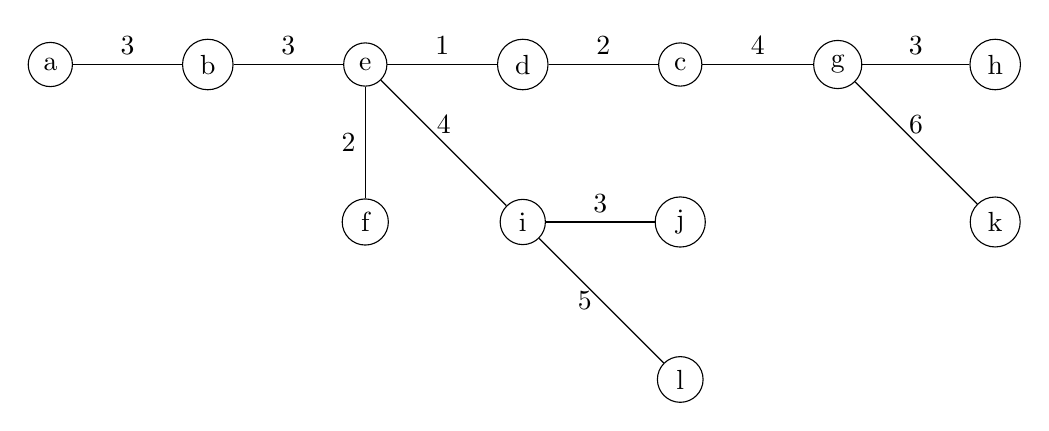
\begin{tikzpicture}
        \node[draw,circle] (a) at (0,0) {a};
        \node[draw,circle] (b) at (2,0) {b};
        \node[draw,circle] (e) at (4,0) {e};
        \node[draw,circle] (d) at (6,0) {d};
        \node[draw,circle] (c) at (8,0) {c};
        \node[draw,circle] (f) at (4,-2) {f};
        \node[draw,circle] (i) at (6,-2) {i};
        \node[draw,circle] (j) at (8,-2) {j};
        \node[draw,circle] (g) at (10,0) {g};
        \node[draw,circle] (h) at (12,0) {h};
        \node[draw,circle] (l) at (8,-4) {l};
        \node[draw,circle] (k) at (12,-2) {k};

        \draw (a) -- node[above] {3} (b);
        \draw (b) -- node[above] {3} (e);
        \draw (e) -- node[above] {1} (d);
        \draw (d) -- node[above] {2} (c);
        \draw (e) -- node[left] {2} (f);
        \draw (e) -- node[above] {4} (i);
        \draw (i) -- node[above] {3} (j);
        \draw (c) -- node[above] {4} (g);
        \draw (g) -- node[above] {3} (h);
        \draw (i) -- node[left] {5} (l);
        \draw (g) -- node[above] {6} (k);
    \end{tikzpicture}
    \caption{Minimum Spanning Tree generated using Kruskal's Algorithm}
\end{figure}




>>>>>>> 9681e1f43439df2f2b411d2e26963757fec5caae
\end{document}